\documentclass[12pt]{article}

\usepackage[english]{babel}
\usepackage[utf8x]{inputenc}
\usepackage{amsmath}
\usepackage{graphicx}
\usepackage[colorinlistoftodos]{todonotes}
\usepackage{listings}
\usepackage{color}
\usepackage{indentfirst}

\definecolor{nGreen}{rgb}{0,0.6,0}
\definecolor{nGray}{rgb}{0.5,0.5,0.5}
\definecolor{nPurple}{rgb}{0.58,0,0.82}
\lstset{ 
  backgroundcolor=\color{white},   
  basicstyle=\footnotesize,       
  breakatwhitespace=false,         
  breaklines=true,                
  captionpos=b,                  
  commentstyle=\color{nGreen},   
  extendedchars=true,             
  frame=false,	                 
  keepspaces=true,                 
  keywordstyle=\color{blue},                  
  numbers=left,                   
  numbersep=5pt,                  
  numberstyle=\tiny\color{nGray}, 
  rulecolor=\color{black},        
  showspaces=false,               
  showstringspaces=false,         
  showtabs=false,                 
  stepnumber=1,                   
  stringstyle=\color{nPurple},    
  tabsize=2,	                  
  title=\lstname                  
}

\title{Diabolic Magic Squares}
\author{Arturo Chinchilla Sánchez, Malcolm Davis Steele}
\begin{document}
\maketitle
%------------------------------------------------------------------------------------------
% 	ABSTRACT
%------------------------------------------------------------------------------------------
\begin{abstract}
"Logic programming and one of its representatives, PROLOG, make a declarative approach to writing computer programs. Logic programs can be understood and studied using two abstract concepts: truth and logical deduction. One can ask whether an axiom in a program is true, under some interpretation of the program symbols, or whether a logical statement is a consequence of the program. These questions can be answered independently of any concrete execution mechanism.

On the contrary, Prolog is a programming language with precise operational meaning that borrows its basic concepts from logic programming. The Prolog programs are instructions for execution on a computer. These instructions can almost always be read as logical statements and, most important, the result of a computation of a Prolog program is a logical consequence of the axioms in it.

Note, that effective Prolog programming requires an understanding of the theory of logic programming".\cite{abstract}
\end{abstract}

%----------------------------------------------------------------------------------------

%---------------------------------------------------------------------------------------
%	CONTENTS AND FIGURES
%---------------------------------------------------------------------------------------
\newpage
\tableofcontents % Prints the main table of contents
\listoffigures % Prints the list of figures

\newpage
%----------------------------------------------------------------------------------------
%  INTRODUCTION
%-----------------------------------------------------------------------------------------
\section{Introduction}

 "A magic square consists of a series of numbers so arranged in a square, that the sum of each row and column and of both the corner diagonals shall be the same amount which may be termed the summation (S). Any square arrangement of numbers that fulfills these conditions may properly be called a magic square." \cite{Andrews}
 
There are several programming paradigms, such as imperative, functional, logic, and others. For this project the logic paradigm will be used. The Logic Paradigm focuses on logic predicates, in which the most important concept is a relation.

"Instead of specifying instructions on a computer, the logic programming paradigm enables the expression of logic. It is therefore useful for dealing with problems where it is not obvious what the functions should be. In this paradigm, programmers specify a set of facts such as statements or relationships that are held to be true, and a set of axioms or rules (i.e., if A is true, then B is true), and use queries to the execution environment to see whether certain relationships hold and to determine the answer by logical inference. This paradigm is popular for database interfaces, expert systems, and mathematical theorem provers"\cite{hitory}.


For this project is created a program composed by two modules, the interface (Frontend) and the logical part (Backend). The Frontend is in charge to interact with the user, gets the user entries and show the information that the user ask. Also handles the communication with the Backend. The logical part is in charge to calculate the user operations, and return to the Frontend the answer.






\newpage
%------------------------------------------------------------------------------------------
% PROBLEM DESCRIPTION 
%------------------------------------------------------------------------------------------
\section{Problem Description}
In this project is proposed to create a program that verifies the user entries and generate diabolic magic squares, using the logic paradigm programming and Prolog  like programming language.
The implementation of this project, is necessary to create 2 programs, that will be interacting with each other.
\begin{itemize}
\item The first part is a Frontend, which purpose will be to interact with the user, take care of the Inputs and Outputs operations and communicates with the second part, the backend.
\item The Backend, contain all the logic part, it's in charge of all the diabolic magic squares resolution.
\end{itemize}
Is allowed develop the Frontend in any language, but the Backend should be developed using Prolog for LINUX. The Backend receive from the Frontend all the request user operations, calculate this, and send the answer again to the Frontend to be displayed to the user.
\subsection{What's a "Diabolic Magic Square"?}
"The Diabolic Magic Square also, known as the Pandiagonal Magic Square, pandiagonal magic square, diabolic square, diabolical square is the one that satisfies the condition that the square should be magic along the broken diagonals as well as along the two ordinary diagonals"\cite{whatis}.
\newline
"In other words, if a Diabolic Magic Square is cut into two pieces along a line between any two rows or any two columns, and the two pieces are interchanged, the real square so formed will also be pandiagonally magic"\cite{whatis}.
See the Figure \ref{DMS}.
\begin{figure}[h!]
 	\centering
  	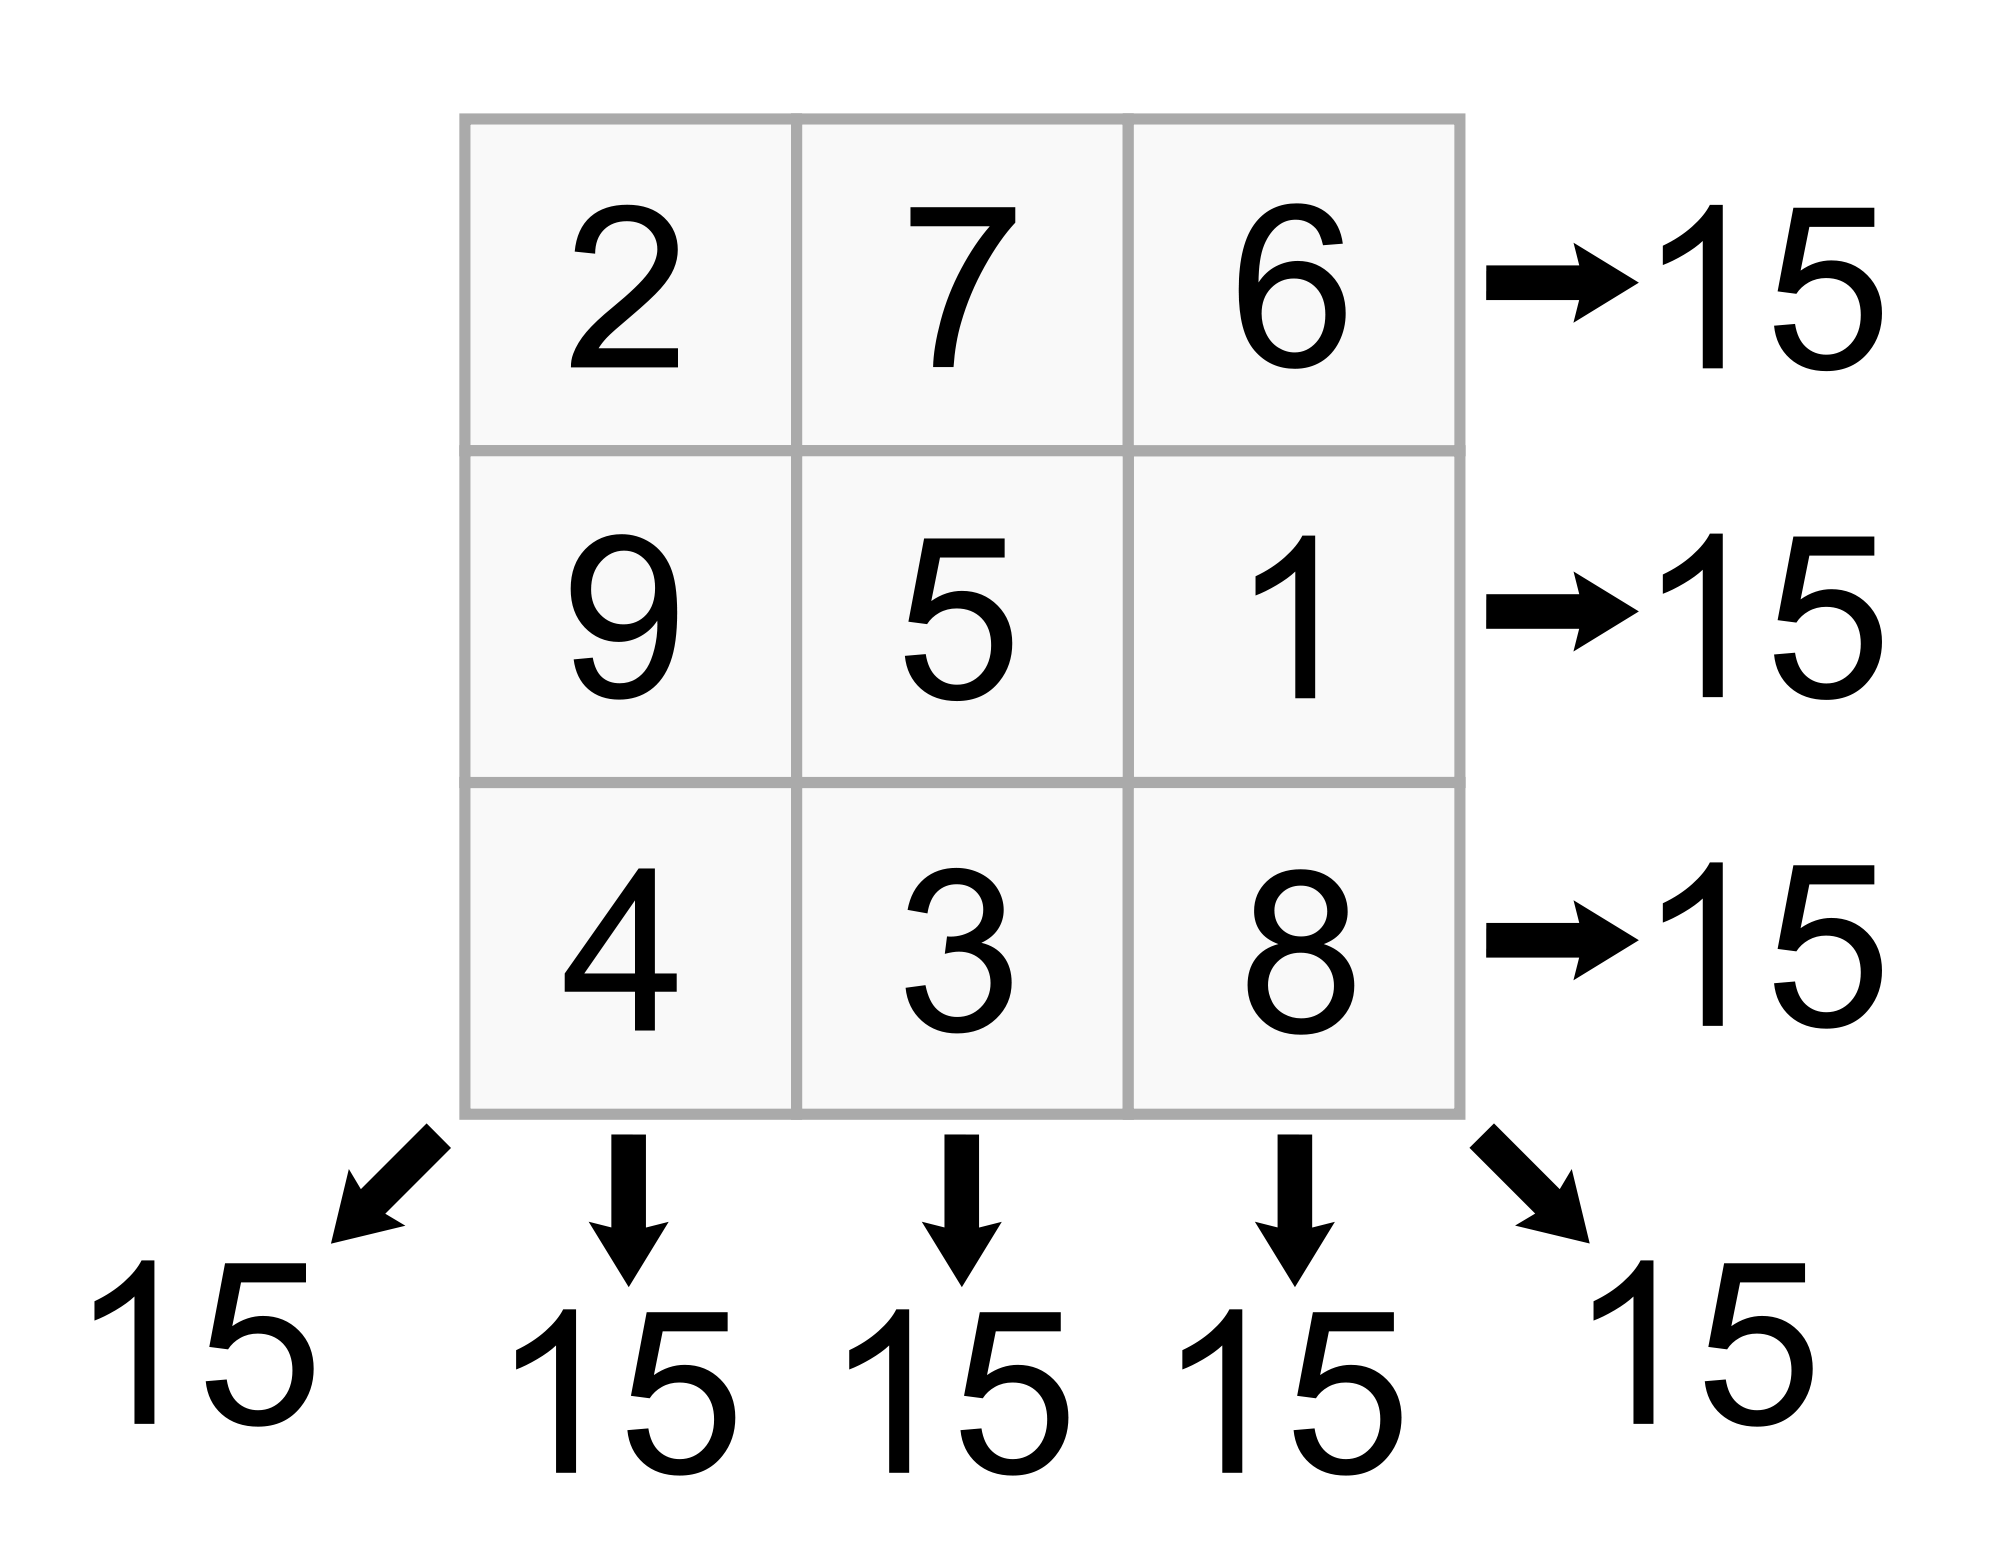
\includegraphics[scale=0.06]
  	{Images/DMS.png}
  	\caption{Diabolic Magic Square 3x3.}
     \label{DMS}
\end{figure}




\newpage
%------------------------------------------------------------------------------------------
% USER GUIDE
%------------------------------------------------------------------------------------------
\section{User Guide}
\subsection{hardware and software requirements}
\begin{itemize}
\item HDD: At least 100MB free.
\item RAM Memory: 2GB.
\item Processor: Dual Core Processor (1.4GHz)
\item OS: Linux Mint 17.2 or another version.
\item IDE: IntelliJ IDEA 
\item Libraries: SWI-Prolog and Java JRE 8.
\end{itemize}

\subsection{How use the program}

\begin{itemize}
\item Open the project with IntelliJ IDEA and run it.
\item When you run the program, a window is displayed, and you have two options, entry your Diabolic Magic Square for the program verifies if is or not, or choose generate with the amount of squares.See the Figure \ref{inter1}

\begin{figure}[h!]
 	\centering
  	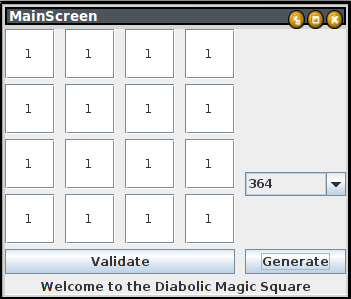
\includegraphics[scale=0.5]
  	{Images/inter1.png}
  	\caption{Principal Program Window .}
     \label{inter1}
\end{figure}

\item If you chose the option that generates squares, the program will be display a window with you request. See the Figure \ref{inter2} and the Figure \ref{inter3}.

\begin{figure}[h!]
 	\centering
  	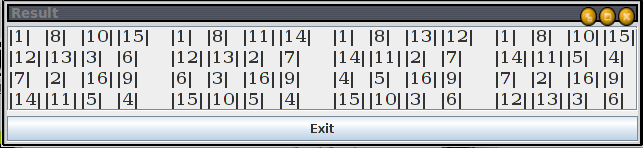
\includegraphics[scale=0.5]
  	{Images/inter2.png}
  	\caption{Window that show four squares.}
     \label{inter2}
\end{figure}

\begin{figure}[h!]
 	\centering
  	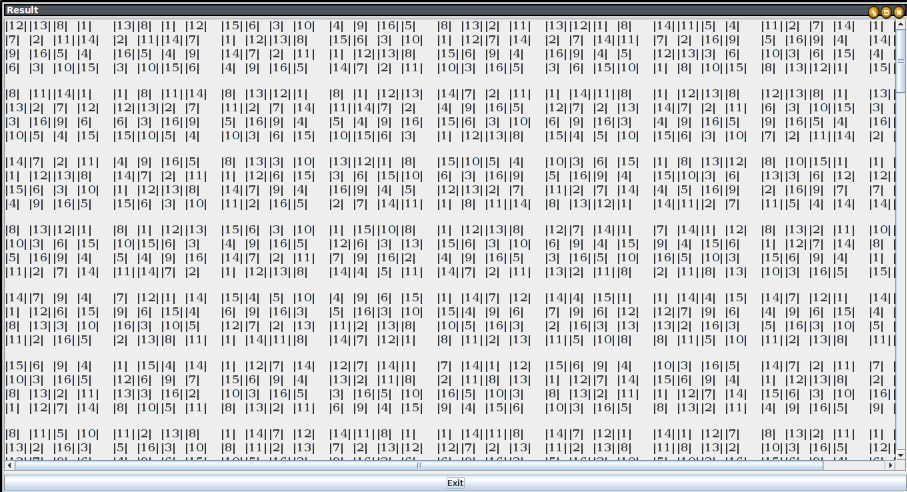
\includegraphics[scale=0.5]
  	{Images/inter3.png}
  	\caption{Window that show all the squares.}
     \label{inter3}
\end{figure}


\end{itemize}




\newpage
%------------------------------------------------------------------------------------------
% DEVELOPMENT ENVIROMENT 
%------------------------------------------------------------------------------------------
\section{Development environment}

\subsection{Git and Github}
To store the code in a practical way and have a versioning control Git is used  for creating repositories and GitHub as service and cloud storage. This code manager (Git) let us to create branches for each member of the group and work separately, change the branch work, see and edit code of another branches, make commits for later if you want to go back in your code and when each part needed is done they can be merged into master branch to have a final version of the code. See Fig \ref{git}
\begin{figure}[h!]
 	\centering
  	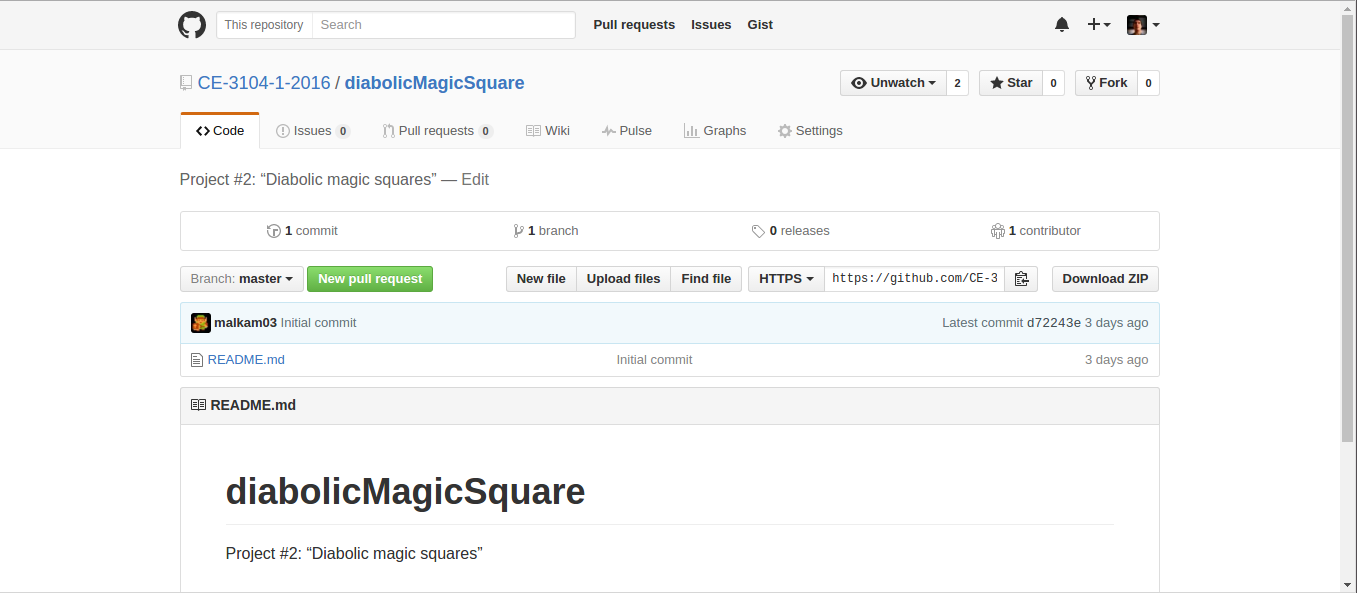
\includegraphics[scale=0.3]
  	{Images/GitHub.png}
  	\caption{GitHub Interface.}
     \label{git}
\end{figure}

\subsection{SublimeText}
It's a text editor for code, markup and prose. It contain functionalities very  useful for programmers and facilitate the code development process. It proved to be very versatile and stable, giving good impressions, simple but with great features. Things like word suggestion, coloring restricted words, minimap, multi selection and multi cursor.Also support multiple languages include Prolog and others like Java, C, C++. See the Figure \ref{Sublime}
\begin{figure}[h!]
 	\centering
  	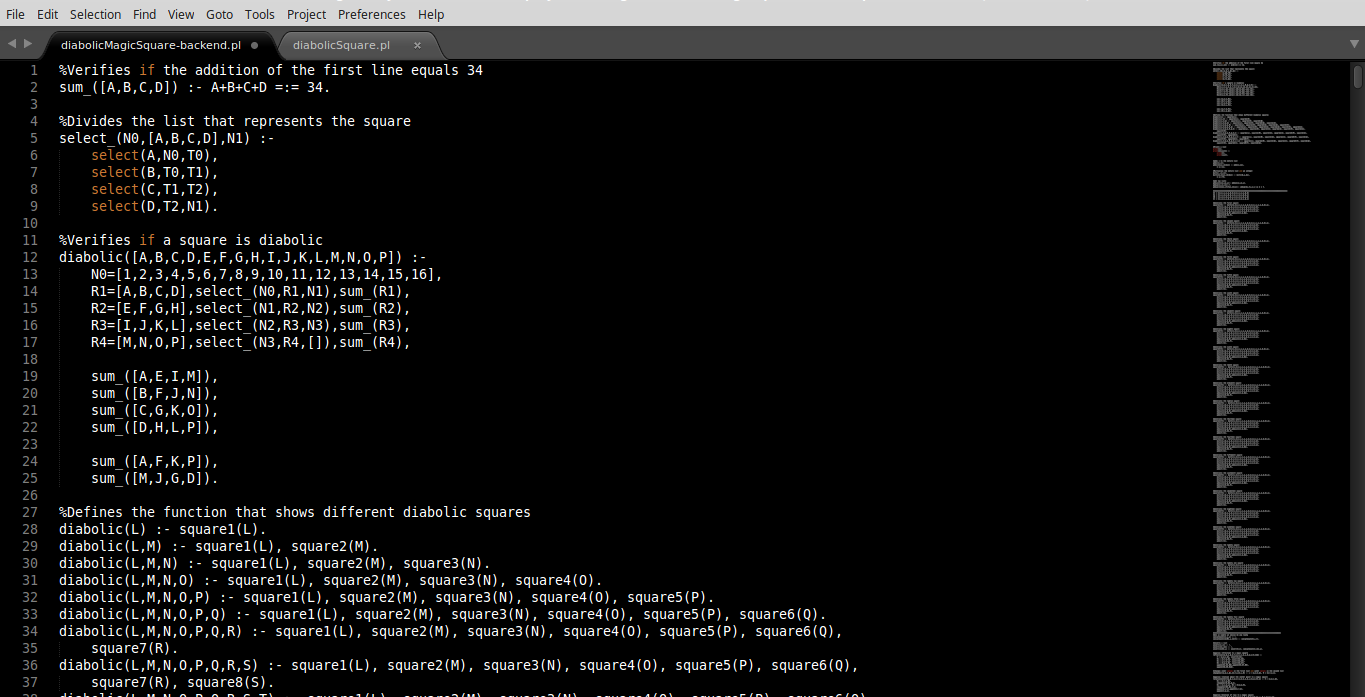
\includegraphics[scale=0.3]
  	{Images/Sublime.png}    
  	\caption{Sublime Text, text editor.}
    \label{Sublime}
\end{figure}

\subsection{Overleaf}
Free online tool used to write academic documents. This service allow create, edit and share your documents easily using \LaTeX. Provide two principal windows, in the first you can write your document, obviously using the \LaTeX syntax, and the second you can see your compiled document. \LaTeX also is composed of a large set of macros getting documents have a typographic high quality. Therefore it is widely used for the creation of academic papers, theses and technical books, since the typographic quality and made with \LaTeX documents is comparable to that of a great scientific publishing. See the Figure \ref{overleaf}
\begin{figure}[h!]
 	\centering
  	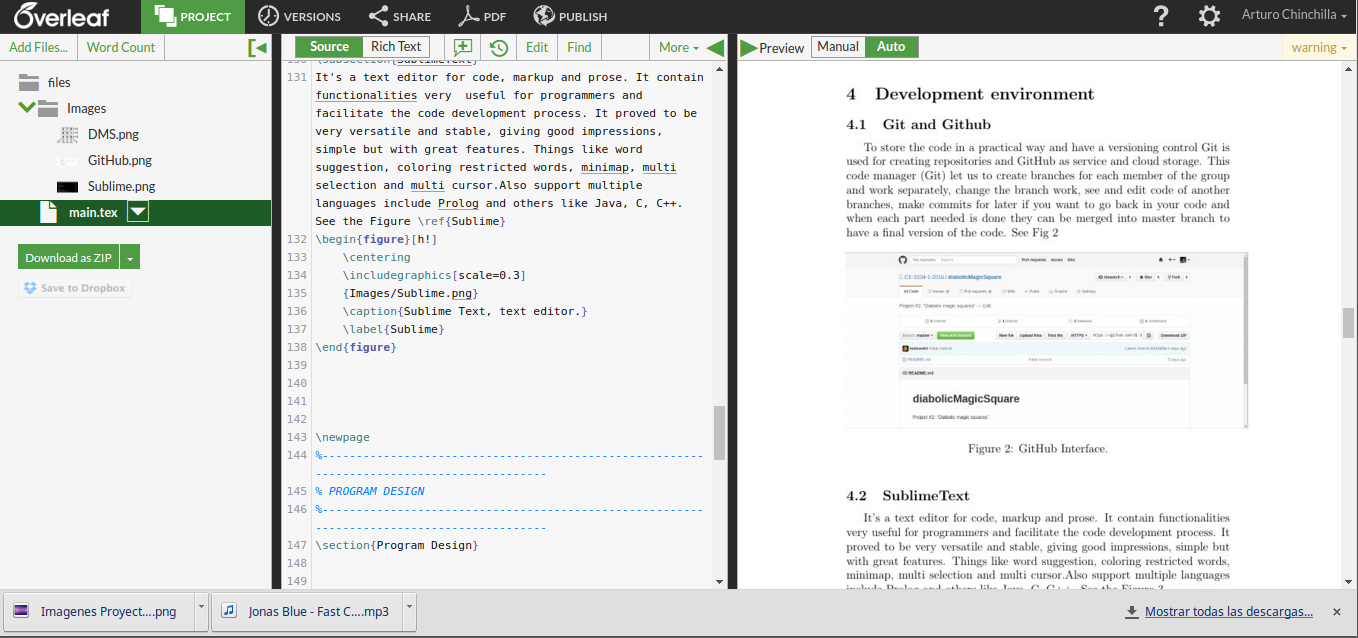
\includegraphics[scale=0.3]
  	{Images/Overleaf.png}
  	\caption{Overleaf Interface Code-Compiled.}
     \label{overleaf}
\end{figure}


\newpage
%------------------------------------------------------------------------------------------
% PROGRAM DESIGN
%------------------------------------------------------------------------------------------
\section{Program Design}
The Backend contains the logical part, it's in charge to check if the user entries is a Magic Square, and generates 384 different Magic Squares based in some Squares stored in the code. But, how is it possible? the squares are generated applying some operations to the matrices that represent the principal squares.
\subsection{Reflection}
The reflection operation consist in change the first column by the last column, generating a new magic square. See the Figure \ref{reflection1} and the Figure \ref{reflection2}
\begin{figure}[h!]
 	\centering
  	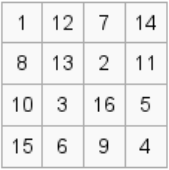
\includegraphics[scale=0.3]
  	{Images/reflection1.png}
  	\caption{Magic Square A.}
     \label{reflection1}
\end{figure}\begin
{figure}[h!]
 	\centering
  	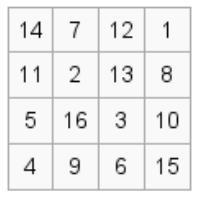
\includegraphics[scale=0.3]
  	{Images/reflection2.png}
  	\caption{Reflection of A.}
     \label{reflection2}
\end{figure}
\subsection{Rotation about the center point}
This operation take the external values around the corners and change this. See the Figure \ref{rotationcenter1} and the Figure \ref{rotationcenter2}
\begin{figure}[h!]
 	\centering
  	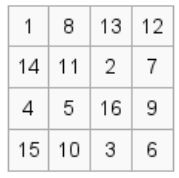
\includegraphics[scale=0.3]
  	{Images/rotationcenter1.png}
  	\caption{Magic Square B.}
     \label{rotationcenter1}
\end{figure}
\begin{figure}[h!]
 	\centering
  	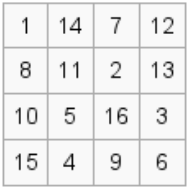
\includegraphics[scale=0.3]
  	{Images/rotationcenter2.png}
  	\caption{Rotation about the center of B.}
 \label{rotationcenter2}
\end{figure}

\subsection{Rotation of Columns}
This operation get and remove the last  column (most right column) and put it on the first place in the square.

\subsection{Rotation of Rows}
This operation get and remove the top row of the square and put it on the bottom place.
\subsection{Convolution}
This operation consist in divide the square in four mini-squares, and rotate those squares. See the Figure \ref{convolution1} and the Figure \ref{convolution2}

\begin{figure}[h!]
 	\centering
  	
\includegraphics[scale=0.3]
  	{Images/convolution1.png}
  	\caption{Magic Square C.}
     \label{convolution1}
\end{figure}
\begin{figure}[h!]
 	\centering
  	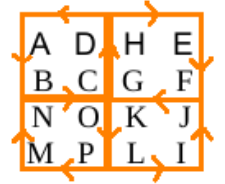
\includegraphics[scale=0.3]
  	{Images/convolution2.png}
  	\caption{Convolution of C.}
 \label{convolution2}
\end{figure}

\subsection{Solution}
"All of the Order 4 Pan-Magic Squares are based on the same underlying "Magic Carpet", a simple pattern consisting of alternating pairs of ones with zeros(See the figure \ref{magicarpet}). Four samples of this pattern are multiplied by 8, 4, 2, and 1, to make the Magic Carpets which are added together to make the final square. The 8, 4, 2, and 1, can be used in any order to make different squares" \cite{solution}.
\begin{figure}[h!]
 	\centering
  	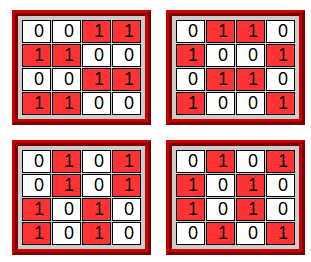
\includegraphics[scale=0.4]
  	{Images/magicarpet.png}
  	\caption{Patterns of zeros and ones.}
 \label{magicarpet}
\end{figure}

This sequence of squares show the production of one square by this technique: Figure \ref{multiplied}

\begin{figure}[h!]
 	\centering
  	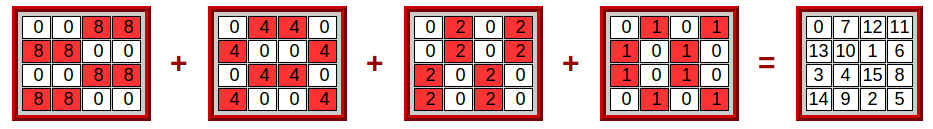
\includegraphics[scale=0.4]
  	{Images/multiplied.png}
  	\caption{Patterns of zeros and ones.}
 \label{multiplied}
\end{figure}

Note: For our project, sum 1 to each value of the squares, because the range of possible values is 1 to 16.

%------------------------------------------------------------------------------------------
% STUDENT ACTIVITY LOG
%------------------------------------------------------------------------------------------
\section{Student Activity Log}
\subsection{Arturo's Time-Sheet}
\begin{center}
\begin{tabular}{ |c|c|c| } 
 \hline
 Date & Task Description & Spent Time \\ 
 \hline\hline
 04/12/2016 & Meeting to divide tasks. & 2 hours\\
 04/12/2016 & Installing SWI-Prolog. & 2 hours\\
 04/12/2016 & Investigation about Prolog syntax & 5 hours\\
 04/13/2016 & Create the verifies entry and auxiliaries & 7 hours\\
 04/13/2016 & Implement the method that creates the principal squares & 8 hours\\
 04/14/2016 & Implement the operations methods & 10 hours\\
 04/14/2016 & Fixing some bugs & 6 hours\\
 04/15/2016 & Create the method showall & 13 hours\\
 04/15/2016 & Documentation starts & 7 hours\\
 \hline
 & Total & 60 hours\\ 
 \hline
\end{tabular}
\end{center}

\subsection{Malcolm's Time-Sheet} 
\begin{center}
\begin{tabular}{ |c|c|c|} 
 \hline
 Date &  Task Description &  Spent Time \\ 
 \hline\hline 
 04/12/2016 & Meeting to divide tasks & 2 hours\\
 04/12/2016 & Installing SWI-Prolog. & 2 hours\\
 04/13/2016 & Investigation about very easy language to connect both & 4 hours\\
 04/13/2016 & Interface beginning using QT & 7 hours\\
 04/14/2016 & Some more investigation about the language & 3 hours\\
 04/14/2016 & Interface beginning again using Java & 8 hours\\
 04/14/2016 & Implement the communication & 6 hours\\
 04/14/2016 & Trying to fix the communication with the backend & 5 hours\\
 04/14/2016 & Trying to fix the communication with the backend & 7 hours\\
 04/15/2016 & Make the last fixes to the interface & 9 hours\\
 04/15/2016 & Documentation starts & 6 hours\\
  \hline
 & Total & 61 hours\\ 
 \hline
\end{tabular}
\end{center}

%------------------------------------------------------------------------------------------
% PROJECT FINAL STATUS
%------------------------------------------------------------------------------------------
\section{Project Final Status.}
The project is completed in a good way, all the functionalities and interface developed successfully, and communication between the two sides also occurs successfully. The interface is friendly with the user and anyone can use it.
\subsection{Issues, Limitations or Challenges}
\begin{itemize}
\item From previous courses we bring the habit of thinking of a same way, but nevertheless in the course of Programming Languages we are forced to learn new paradigms, and thus think of a different way to solve computational problems , the difficulty of learning to think in a differently way (new programming paradigm), in addition to learning a new language with its syntax, semantics and pragmatics.
\item Choose the correct Programming language that functions in conjunction with Prolog was a very hard decision, all the investigation and the time of testing and error.
\item Connect the Backend with the Frontend was difficult, because both was developed on different programming languages, and for this many times the languages behavior wasn't correct..
\end{itemize}
\subsection{known Issues}
\begin{itemize}
\item When one square is requested for the user, the program takes some time to respond to the request,for that reason the option is disabled on the interface.
\end{itemize}

%------------------------------------------------------------------------------------------
% Conclusions, Suggestions and Recommendations
%------------------------------------------------------------------------------------------
\section{Conclusions, Suggestions and Recommendations.}
\begin{itemize}
\item Tools like the handler code versions is very useful, because in case of any failure in the new version allows us to return to a previous, plus the possibility of linking it to the storage service in the cloud, to share, and work together in a very easy way.
\item Sublime Text can be one of the better text editors, that should not make lack in the programmer's computer, for its flexibility and support for multiple programming languages, in addition to the vast amount of functionalities adapted for this use.
\item Connect the Frontend with the Backend wasn't easy, because use two different language make it difficult, the only way is use external libraries that help with this task. 
\end{itemize}

%--------------------------------------------------------------------------------
%             References
%--------------------------------------------------------------------------------

\begin{thebibliography}{10}
\bibitem{abstract}
  R.  Barták,
  \emph{"Prolog Guide - Introduction"}
  Kti.ms.mff.cuni.cz,
  1998. [Online].
 Available: http://kti.ms.mff.cuni.cz/~bartak/prolog/intro.html. 
 [Accessed: 13- Apr- 2016].
 
 \bibitem{Andrews}
  W. Andrews,
  \emph{"Magic squares and cubes"}
  New York: Dover Publications,
  1960, p. 1.
 
 \bibitem{whatis}
  \emph{"Math Logic - Diabolic Magic Square"}
  Calculatoredge.com,
  2008. [Online]. Available:   	    		http://www.calculatoredge.com/math/mathlogic/logicans22.htm. 
  [Accessed: 16- Apr- 2016].
 

 \bibitem{solution}
  \emph{"The 4x4 Pan-Magic Squares"}
   Grogono.com,
   2010. [Online]. 
   Available: http://www.grogono.com/magic/4x4.php. 
   [Accessed: 16- Apr- 2016].
 
 \bibitem{hitory}
  \emph{"Past programming languages and their influences on today's languages and programming paradigms - Engineering and Technology History Wiki"}
   Ethw.org,
   2015. [Online]. 
   Available: http://ethw.org/Past\_programming\_languages\_and\_their\_influences\_on\_today's\_languages\_and\_programming\_paradigms. 
   [Accessed: 16- Apr- 2016].
 
 


 


\end{thebibliography}
\end{document}